% !TEX root = ../main.tex
%

\part{最適化}

\chapter{導入}

この部では,最適化のアルゴリズムをまとめる.

最適化問題は一般に次のように書ける.

\begin{align}\label{eq:optimization_general_problem}
    \text{minimize} \hspace{1em} & f(\bm{x})                 \\
    \text{s.t.} \hspace{1em}     & \bm{g}(\bm{x}) \le \bm{0} \\
                                 & \bm{h}(\bm{x}) = \bm{0}
\end{align}

ここで,
$\bm{x} \in \setR^n$,
$f : \setR^n \to \setR$,
$\bm{g} : \setR^n \to \setR^m$,
$\bm{h} : \setR^n \to \setR^r$
とする.
また,ベクトル同士の「$\le$」による比較は
全ての要素において「$\le$」の関係が成り立つことを意味する.

問題\eqref{eq:optimization_general_problem}において,
関数$f$は目的関数,
$\bm{g}(\bm{x}) \le \bm{0}$, $\bm{h}(\bm{x}) = \bm{0}$は制約条件と呼ばれ,
制約条件を満たす中で目的関数を最小化する問題を示している.
最小化した結果の変数 $\bm{x}$ は最適解と呼ばれ,
目的関数の値は最適値と呼ばれる.

なお,最小化でなく最大化で定式化する場合もあるが,
ここでは最小化に統一して説明する.

最適化のアルゴリズムは,
対称とする問題に制約条件があるものとないものに分けられる.

\chapter{基本的な定義と性質}

\begin{definition}[{\cite[Section 6.4]{Luenberger2003}},{\cite[Section 3.1.1]{Boyd2004}}]
    関数 $f : \setR^n \to \setR$ が
    $\forall \bm{x}, \bm{y} \in \setR^n$, $\forall \alpha \in [0, 1]$ に対して
    \begin{equation}
        f\left(\alpha \bm{x} + (1-\alpha) \bm{y}\right)
        \le \alpha f(\bm{x}) + (1-\alpha) f(\bm{y})
    \end{equation}
    を満たす場合,関数 $f$ を凸関数(convex function)と呼ぶ.
\end{definition}

\begin{theorem}[{\cite[Section 6.4]{Luenberger2003}},{\cite[Section 3.1.3]{Boyd2004}}]
    $C^1$ 級関数 $f : \setR^n \to \setR$ が凸関数であるための必要十分条件は
    $\forall \bm{x}, \bm{y} \in \setR^n$ に対して
    \begin{equation}
        f(\bm{y}) \ge f(\bm{x}) + \nabla f(\bm{x})^\top (\bm{y} - \bm{x})
    \end{equation}
    が成り立つことである.
\end{theorem}

\begin{theorem}[{\cite[Section 6.4]{Luenberger2003}},{\cite[Section 3.1.3]{Boyd2004}}]
    $C^2$ 級関数 $f : \setR^n \to \setR$ が凸関数であるための必要十分条件は
    $\forall \bm{x} \in \setR^n$ に対して
    \begin{equation}
        \nabla^2 f(\bm{x}) \succeq O
    \end{equation}
    が成り立つことである.
\end{theorem}

\begin{definition}[{\cite[Section 6.4]{Luenberger2003}},{\cite[Section 3.1.1]{Boyd2004}}]
    関数 $f : \setR^n \to \setR$ が
    $\forall \bm{x}, \bm{y} \in \setR^n$, $\forall \alpha \in [0, 1]$ に対して
    \begin{equation}
        f\left(\alpha \bm{x} + (1-\alpha) \bm{y}\right)
        < \alpha f(\bm{x}) + (1-\alpha) f(\bm{y})
    \end{equation}
    を満たす場合,関数 $f$ は狭義凸関数(strictly convex function)であるという.
\end{definition}

\begin{definition}[{\cite[Section 9.1.2]{Boyd2004}}]
    $C^2$ 級関数 $f : \setR^n \to \setR$ が
    ある定数 $m > 0$ を持ち,
    $\forall \bm{x} \in \setR^n$ に対して
    \begin{equation}
        \nabla^2 f(\bm{x}) \succeq m I
    \end{equation}
    を満たす場合,関数 $f$ は強凸関数(strongly convex function)であるという.
\end{definition}

\begin{theorem}[{\cite[Section 9.1.2]{Boyd2004}}]
    $C^2$ 級関数 $f : \setR^n \to \setR$ が強凸関数である場合,
    $\forall \bm{x}, \bm{y} \in \setR^n$ に対して
    \begin{equation}
        f(\bm{y}) \ge f(\bm{x}) + \nabla f(\bm{x})^\top (\bm{y} - \bm{x})
        + \frac{m}{2} \| \bm{y} - \bm{x} \|_2^2
    \end{equation}
    が成り立つ.
\end{theorem}

\begin{theorem}[{\cite[Section 9.1.2]{Boyd2004}}]
    $C^2$ 級関数 $f : \setR^n \to \setR$ が強凸関数である場合,
    関数 $f$ が最小となる $\bm{x} \in \setR^n$ は一意的に定まる.
\end{theorem}

% !TEX root = ../main.tex
%

\section{1 次元における解法}

1 次元の変数 $x \in \setR$ における関数 $f : \setR \to \setR$ の最小化においては,
比較的簡単なアルゴリズムが存在する.

\subsection{黄金比探索}

黄金比探索 (golden section search, \cite[10.2]{Press2007}) では,
区間を黄金比で分割していきながら最適解を探索する.

まず,区間 $[a,b]$ に対して中間点 $c$ を
\begin{equation}
    \frac{c - a}{b - a} = \omega
\end{equation}
の比でとる($0 < \omega < 1/2$).そして,$c$ と対称な位置に点 $d$ をとる.つまり,
\begin{equation}
    \frac{b - d}{b - a} = \omega
\end{equation}
とする.このとき,
\begin{equation}
    \frac{d - a}{b - a} = 1 - \frac{b - d}{b - a} = 1 - \omega
\end{equation}
である.ここで,
\begin{itemize}
    \item $f(c) < f(d)$ となった場合,最適解を探索する区間を $[a, b]$ から $[a, d]$ に更新する.
    \item $f(c) > f(d)$ となった場合,最適解を探索する区間を $[a, b]$ から $[c, b]$ に更新する.
\end{itemize}
のようにし,更新後の区間における中間点の相対位置が
区間 $[a, b]$ における点 $c$ と変わらないようにするため以下の方程式を立てる.
\begin{align}
    \frac{d - c}{d - a} &= \omega, &
    \frac{d - c}{b - c} &= \omega
\end{align}
$b - a$ に対する比を用いることで,どちらも
\begin{align}
    \frac{1 - 2\omega}{1 - \omega} &= \omega
\end{align}
と変形でき,これを $0 < \omega < 1/2$ の制限のもとで解くと
\begin{equation}
    \omega = \frac{3 - \sqrt{5}}{2} \approx 0.3819660112501052
\end{equation}
となる.
なお,このアルゴリズムの区間の分割において,以下のように黄金比が登場する.
\begin{equation}
    \frac{b - a}{b - c} = \frac{1}{1 - \omega} = \frac{1 + \sqrt{5}}{2} \approx 1.618033988749895
\end{equation}

% !TEX root = ../main.tex
%

\chapter{勾配を用いた制約なし最適化}

ここでは,勾配を用いた最適化アルゴリズムをまとめる.

\begin{algorithm}[tp]
    \caption{勾配による最適化}
    \label{alg:optimization_unconstrained_descent-methods_general-descent-method}
    \begin{algorithmic}
        \Procedure{DescentMethod}{$f, \bm{x}_0$}
            \For{$i = 1,2,\ldots$}
                \State 更新方向 $\bm{d}_i \in \setR^n$ を算出する
                \State 直線探索により更新方向に掛ける係数 $t_i$ を決定する
                \Comment{通常 $f(\bm{x}_{i-1} + t_i \bm{d}_i) < f(\bm{x}_{i-1})$ とする}
                \State $\bm{x}_i \gets \bm{x}_{i-1} + t_i \bm{d}_i$
                \If{終了条件を満たしている}
                    \State \Return $\bm{x}_i$
                \EndIf
            \EndFor
        \EndProcedure
    \end{algorithmic}
\end{algorithm}

勾配を用いた最適化アルゴリズムでは,
一般に
Algorithm \ref{alg:optimization_unconstrained_descent-methods_general-descent-method}
のような手順で反復的に最適化を進めていく.
更新方向の算出方法により,
最急降下法,Newton 法,共役勾配法のような様々なアルゴリズムが存在する.

\section{直線探索}

まずは,直線探索の方法をまとめる.
直線探索では
$\nabla f(\bm{x}_{i-1})^\top \bm{d}_i < 0$ となっている
(つまり,$\bm{d}_i$ は目的関数が減少する方向になっている)
ことを前提とする.

直線探索の方法として,以下のような方法が挙げられる.

\begin{itemize}
    \item 厳密直線探索
    \item Backtracking line search
\end{itemize}

厳密直線探索は,更新後の目的関数の値
$f(\bm{x}_{i-1} + t_i \bm{d}_i)$
が最小となる $t_i$ を探索する.

\begin{algorithm}[tp]
    \caption{Backtracking Line Search \cite[Section 9.2]{Boyd2004}}
    \label{alg:optimization_unconstrained_descent-methods_BacktrackingLineSearch}
    \begin{algorithmic}
        \Procedure{BacktrackingLineSearch}{$f, \bm{x}_{i-1}, \bm{d}_i$}
            \State $t_i \gets 1$
            \While{$f(\bm{x}_{i-1} + t_i \bm{d}_i) > f(\bm{x}_{i-1}) + \alpha t_i \nabla f(\bm{x}_{i-1})^\top \bm{d}_i$}
                \State $t_i \gets \beta t_i$
            \EndWhile
        \EndProcedure
    \end{algorithmic}
\end{algorithm}

\begin{figure}[tp]
    \centering
    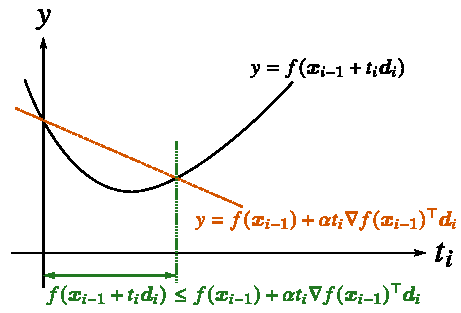
\includegraphics[width=0.7\linewidth]{optimization/Armijo-rule-image.pdf}
    \caption{Armijo の条件(式\eqref{eq:optimization_unconstrained_descent-methods_Armijo-rule})のイメージ}
    \label{fig:optimization_unconstrained_descent-methods_Armijo-rule-image}
\end{figure}

Backtracking Line Search \cite[Section 9.2]{Boyd2004} は
Armijo の条件 \cite[Section 7.5]{Luenberger2003}
\begin{equation}
    f(\bm{x}_{i-1} + t_i \bm{d}_i) \le f(\bm{x}_{i-1}) + \alpha t_i \nabla f(\bm{x}_{i-1})^\top \bm{d}_i
    \label{eq:optimization_unconstrained_descent-methods_Armijo-rule}
\end{equation}
を利用する.
ここで,$\alpha$ は $\alpha \in (0,1)$ を満たす定数であり,
Armijo の条件は,
図\ref{fig:optimization_unconstrained_descent-methods_Armijo-rule-image}のように
十分小さい $t_i$ を選択するための条件となっている.
Backtracking Line Search では,
$\alpha \in (0, 1/2)$ とし,
Algorithm \ref{alg:optimization_unconstrained_descent-methods_BacktrackingLineSearch}
のように
$t_i$ を初期値 1 から $\beta \in (0, 1)$ 倍していき,
式 \eqref{eq:optimization_unconstrained_descent-methods_Armijo-rule} を満たすものを探索する.
一般に,パラメータ $\alpha$, $\beta$ は
$\alpha \in [0.01, 0.3]$, $\beta \in [0.1, 0.8]$ の範囲で設定される
\cite[Section 9.2]{Boyd2004}.

\section{最急降下法}

最急降下法では,更新方向を $\bm{d}_i = -\nabla f(\bm{x}_{i-1})$ とする.
確実に目的関数の減少する方向を示しており,
ここで示す他のアルゴリズムよりも更新方向の算出が簡単である.
目的関数が強凸関数である場合において,
最適解への収束が証明されている
\cite[Section 9.3.1]{Boyd2004}.

\section{Newton 法}

Newton 法では,
目的関数が狭義凸関数である(つまり,Hessian $\nabla^2 f(\bm{x}_{i-1})$ が正定値である)場合を対象とし,
更新方向を
$\bm{d}_i = -\nabla^2 f(\bm{x}_{i-1})^{-1} \nabla f(\bm{x}_{i-1})$
とする.
$\nabla^2 f(\bm{x}_{i-1})$ が正定値である場合,
$\nabla^2 f(\bm{x}_{i-1})^{-1}$ も正定値になる
\footnote{%
対称行列 $A$ が正定値である場合,$A$ の固有値は正の実数である.%
$A$ は固有値分解により $A=VDV^\top$ ($D$ は固有値による対角行列,$V$ は直交行列)と書くことができるため,%
$A^{-1} = VD^{-1}V^\top$ となる.%
よって,$A^{-1}$ の固有値も全て正の実数であり,%
$A^{-1}$ は正定値である.%
}
ため,
最適解でない $\bm{x}_{i-1}$ においては
$\nabla f(\bm{x}_{i-1})^\top \bm{d}_i = -\nabla f(\bm{x}_{i-1})^\top \nabla^2 f(\bm{x}_{i-1})^{-1} \nabla f(\bm{x}_{i-1}) < 0$
となり,目的関数が減少する方向になっていることを確認できる.
Newton 法の収束性については \cite[Section 9.5.3, 9.6.4]{Boyd2004} にて議論されている.

\section{準 Newton 法}

Newton 法では,
Hessian $\nabla^2 f(\bm{x}_{i-1})$ の逆行列が必要になるが,
$x^4$ のように 2 階微分が 0 になる点があったり,
Hessian の逆行列を安定的に計算できない点があったりする場合には使用できない.
そこで,Newton 法の更新方向
$\bm{d}_i = -\nabla^2 f(\bm{x}_{i-1})^{-1} \nabla f(\bm{x}_{i-1})$
における Hessian を
$\bm{d}_i = -H_{i-1} \nabla f(\bm{x}_{i-1})$
のように Hessian の代わりの行列で置き換える準 Newton 法と呼ばれるアルゴリズムがある.

準 Newton 法のうち,
Davidon-Fletcher-Powell (DFP) 公式では次のように $H_i$ を算出する
\cite[Section 9.3]{Luenberger2003}, \cite[Section 10.9]{Press2007}.
\begin{align}
    H_{i+1} &= H_i + \frac{\bm{p}_i \bm{p}_i^\top}{\bm{p}_i^\top \bm{q}_i}
        - \frac{H_i \bm{q}_i \bm{q}_i^\top H_i}{\bm{q}_i^\top H_i \bm{q}_i} \\
    \bm{p}_i &= \bm{x}_{i+1} - \bm{x}_i \\
    \bm{q}_i &= \nabla f(\bm{x}_{i+1}) - \nabla f(\bm{x}_i)
\end{align}
初期値 $H_0$ を対称な正定値の行列にしておけば,
全ての $H_i$ が帰納的に正定値になる
\cite[Section 9.3]{Luenberger2003}.
$H_i$ が正定値であれば,更新方向 $\bm{d}_i$ は目的関数の減少する方向になる.

また,同様の性質を持つ公式の 1 つとして,
Broyden-Fletcher-Goldfarb-Shanno (BFGS) 公式が存在する
\cite[Section 9.4]{Luenberger2003}.
\begin{align}
    H_i &= B_i^{-1} \\
    B_{i+1} &= B_i + \frac{\bm{q}_i \bm{q}_i^\top}{\bm{q}_i^\top \bm{p}_i}
        - \frac{B_i \bm{p}_i \bm{p}_i^\top B_i}{\bm{p}_i^\top B_i \bm{p}_i}
\end{align}
逆行列を計算することで次のようにも書くことができる
\cite[Section 10.9]{Press2007}.
\begin{align}
    H_{i+1} &= H_i + \frac{\bm{p}_i \bm{p}_i^\top}{\bm{p}_i^\top \bm{q}_i}
        - \frac{H_i \bm{q}_i \bm{q}_i^\top H_i}{\bm{q}_i^\top H_i \bm{q}_i}
        + \bm{q}_i^\top H_i \bm{q}_i \bm{v}_i \bm{v}_i^\top \\
    \bm{v}_i &= \frac{\bm{p}_i}{\bm{p}_i^\top \bm{q}_i}
        - \frac{H_i \bm{q}_i}{\bm{q}_i^\top H_i \bm{q}_i}
\end{align}

\section{共役勾配法}

共役勾配法では,
\begin{align}
    \bm{d}_1 &= -\nabla f(\bm{x}_{i-1}) \\
    \bm{d}_i &= -\nabla f(\bm{x}_{i-1}) + \gamma_i \bm{d}_{i-1} \\
    \gamma_i &=
        \frac{(\nabla f(\bm{x}_{i-1}) - \nabla f(\bm{x}_{i-2}))^\top \nabla f(\bm{x}_{i-1})}
        {\|\nabla f(\bm{x}_{i-2})\|_2^2}
\end{align}
のように更新方向を算出する
\cite[Section 8.6]{Luenberger2003}.
$\gamma_i$ については複数の形式があるが,
ここで示している Polak-Ribiere 法は一般により良い結果が得られるという
\cite[Section 8.6]{Luenberger2003}, \cite[Section 10.8]{Press2007}.
Newton 法では計算量の多い逆行列の計算が必要だが,
共役勾配法では計算量が変数の次元のオーダーに収まるため,
各反復の計算時間を抑えられる.

% !TEX root = ../main.tex
%

\section{Downhill Simplex 法}

\begin{algorithm}[tp]
    \caption{Downhill simplex 法}
    \label{alg:optimization_unconstrained_downhill-simplex_downhill-simplex}
    \begin{algorithmic}
        \Procedure{DownhillSimplex}{$f, \bm{x}_0$}
            \State 変数の次元を $n$ とし,$n$ 次元の単体を構成する
                $n + 1$ 個の点 $\bm{x}_0, \ldots, \bm{x}_{n}$ を決定する.
            \Loop
                \State 単体における最大値以外の点からなる超面に対して対称な位置に最大値の点を移動する
                \Comment Reflection
                \If{移動した点の関数値が他の全ての点より小さい場合}
                    \State 最大値の点を超面から離す
                    \Comment Reflection and expansion
                \ElsIf{移動した点がまだ最大値のままである場合}
                    \State 最大値の点を超面に近づける
                    \Comment Contraction
                    \If{移動した点がまだ最大値のままである場合}
                        \State 最小値以外の全ての点を最小値に近づける
                        \Comment Multiple contraction
                    \EndIf
                \Else
                    \State Reflection のみでこの反復における移動を完了する
                \EndIf
                \If{停止条件を満たしている場合}
                    \State \Return
                \EndIf
            \EndLoop
        \EndProcedure
    \end{algorithmic}
\end{algorithm}

Downhill simplex 法 \cite{Press2007} では,
Algorithm \ref{alg:optimization_unconstrained_downhill-simplex_downhill-simplex} のように
変数の空間における単体 (simplex) をルールに沿って反復的に動かしていくことで
関数の最小値を求める手法である.
関数値の大小のみで決まるため,関数の微分がなくとも最適化ができる.

% !TEX root = ../main.tex
%

\chapter{大域最適化}

勾配を用いた最適化アルゴリズムでは、
局所的に目的関数が周りより小さい点(局所最適解)を見つけられるが、
目的関数が最も小さくなる点(大域最適解)を見つけられるとは限らない。
そこで、大域最適解を求める大域最適化のアルゴリズムが考えられている。
本章では大域最適化のアルゴリズムについてまとめる。

\section{Dividing Rectangles (DIRECT) 法}

Dividing Rectangles (DIRECT) 法 \cite{Jones1993} では、
黄金比探索(第 \ref{sec:optimization_golden-section-search} 節)と同様に
領域を分割していきながら最適解を求める。
ただし、黄金比探索と異なり大域最適解を求めるため、
目的関数の値が小さくない点も一定の条件でさらに分割していく。

DIRECT 法では、
探索領域を $n$ 次元単位超立方体 $[0, 1]^n$ とし、
その上で定義される目的関数 $f : [0, 1]^n \to \setR$ を考える。
目的関数は Lipschitz 連続であるとする。
つまり、ある定数 $K$ が存在し、
任意の点 $\bm{x}, \bm{y} \in [0, 1]^n$ について
\begin{equation}
    |f(\bm{x}) - f(\bm{y})| \le K \|\bm{x} - \bm{y}\|_2
\end{equation}
が成り立つとする。
アルゴリズムの進行とともに探索領域は超短形
\footnote{ここで扱う超短形 (hyper-rectangle) は%
$[a_1, b_1] \times [a_2, b_2] \times \ldots \times [a_n, b_n]$%
のように区間の積で示される領域である。}
に分割されていくが、次に分割する超短形を決定するために、
次のような「最適な可能性のある超短形」を定義する。

\begin{definition}[{\cite[Definition 4.1.]{Jones1993}}]
    \label{def:optimization_direct_potentially-optimal}
    反復により探索領域が $m$ 個の超短形に分割されているものとし、
    $i$ 番目の超短形の中心点を $\bm{c}_i$ とする。
    $j$ 番目の超短形が次の条件を満たすような定数 $\tilde{K}$ が存在する場合、
    最適な可能性のある超短形と呼ぶ。
    \begin{align}
        f(\bm{c}_j) - \tilde{K} d_j &\le f(\bm{c}_i) - \tilde{K} d_i & \text{for all $i = 1, \ldots, m$}
        \label{eq:optimization_direct_potentially-optimal_smaller-than-others}
        \\
        f(\bm{c}_j) - \tilde{K} d_j &\le f_{\text{min}} - \epsilon |f_{\text{min}}|
        \label{eq:optimization_direct_potentially-optimal_smaller-than-now}
    \end{align}
    ここで、$f_{\text{min}} = \min{\{f_i \mid i = 1, \ldots, m\}}$ であり、
    $d_i$ は $i$ 番目の超短形の中心から端点までの距離であり、
    $\epsilon$ は正の実数の定数である。
\end{definition}

$f(\bm{c}_j) - \tilde{K} d_j$ は
Lipschitz 定数が $\tilde{K}$ である場合に $j$ 番目の超短形の中で取り得る最小値を示す。
そのため、
式 \eqref{eq:optimization_direct_potentially-optimal_smaller-than-others} は、
Lipschitz 定数が $\tilde{K}$ である場合に
最も小さい値を取り得る超短形が $j$ 番目の超短形であることを示す。
式 \eqref{eq:optimization_direct_potentially-optimal_smaller-than-now} は、
Lipschitz 定数が $\tilde{K}$ である場合に、
$j$ 番目の超短形で現状の大域最適解を
少なくとも $\epsilon |f_{\text{min}}|$ だけ更新する可能性があることを示す。

\begin{figure}[tp]
    \centering
    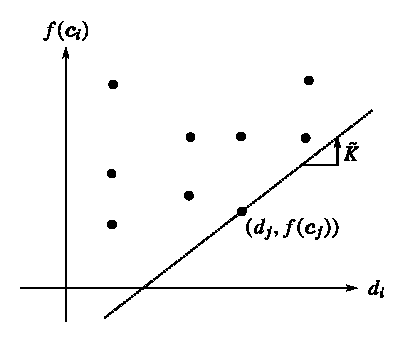
\includegraphics[width=0.7\linewidth]{optimization/DIRECT-potentially-optimal.pdf}
    \caption{式 \eqref{eq:optimization_direct_potentially-optimal_smaller-than-others_rewritten} のイメージ}
    \label{fig:optimization_direct_potentially-optimal_smaller-than-others-image}
\end{figure}

超短形を分割する場合、
各軸の区間の長さを比べて長い方向から分割するようにし、
最も長い軸が複数ある場合は次元の小さい方から順に分割することで、
分割数の同じ超短形は同じ形状になるようにする。
これにより、分割数の同じ超短形は
定義 \ref{def:optimization_direct_potentially-optimal} における $d_i$ が同じになり、
分割数の同じ超短形同士では
式 \eqref{eq:optimization_direct_potentially-optimal_smaller-than-others}
が単に目的関数の大小により評価できるようになる。
また、式 \eqref{eq:optimization_direct_potentially-optimal_smaller-than-others} は
\begin{equation}
    f(\bm{c}_i) \ge f(\bm{c}_j) + \tilde{K} (d_i - d_j)
    \label{eq:optimization_direct_potentially-optimal_smaller-than-others_rewritten}
\end{equation}
のように書くこともでき、
図 \ref{fig:optimization_direct_potentially-optimal_smaller-than-others-image}
のように他の点が全て上に来るような直線を引けることを示す。
このような点を探すアルゴリズムは凸包探索として知られる。

\begin{algorithm}[tp]
    \caption{DIRECT 法}
    \label{alg:optimization_direct}
    \begin{algorithmic}
        \Procedure{DIRECT}{$f, ,\epsilon$}
            \State 単位超立方体 $[0, 1]^n$ を最初の超短形とする
            \Loop
                \State 凸包探索を用いて
                    式 \eqref{eq:optimization_direct_potentially-optimal_smaller-than-others_rewritten}
                    を満たす超短形を探索する
                \State 式 \eqref{eq:optimization_direct_potentially-optimal_smaller-than-now}
                    を満たさない超短形は除外する
                \State 残った超短形を最も長い軸に沿って 3 つに分割する
                \If{停止条件を満たす場合}
                    \State \Return
                \EndIf
            \EndLoop
        \EndProcedure
    \end{algorithmic}
\end{algorithm}

ここまでの議論により、DIRECT 法は
Algorithm \ref{alg:optimization_direct} のようになる。
停止条件としては、反復回数が用いられる。

DIRECT 法の派生としては以下のようなものが挙げられる。

\begin{itemize}
    \item 各局所最適解への収束に重点をおいた DIRECT-l \cite{Gablonsky2001}
\end{itemize}

